\documentclass{standalone}
\usepackage{tikz}
\usetikzlibrary{patterns, positioning}

\begin{document}
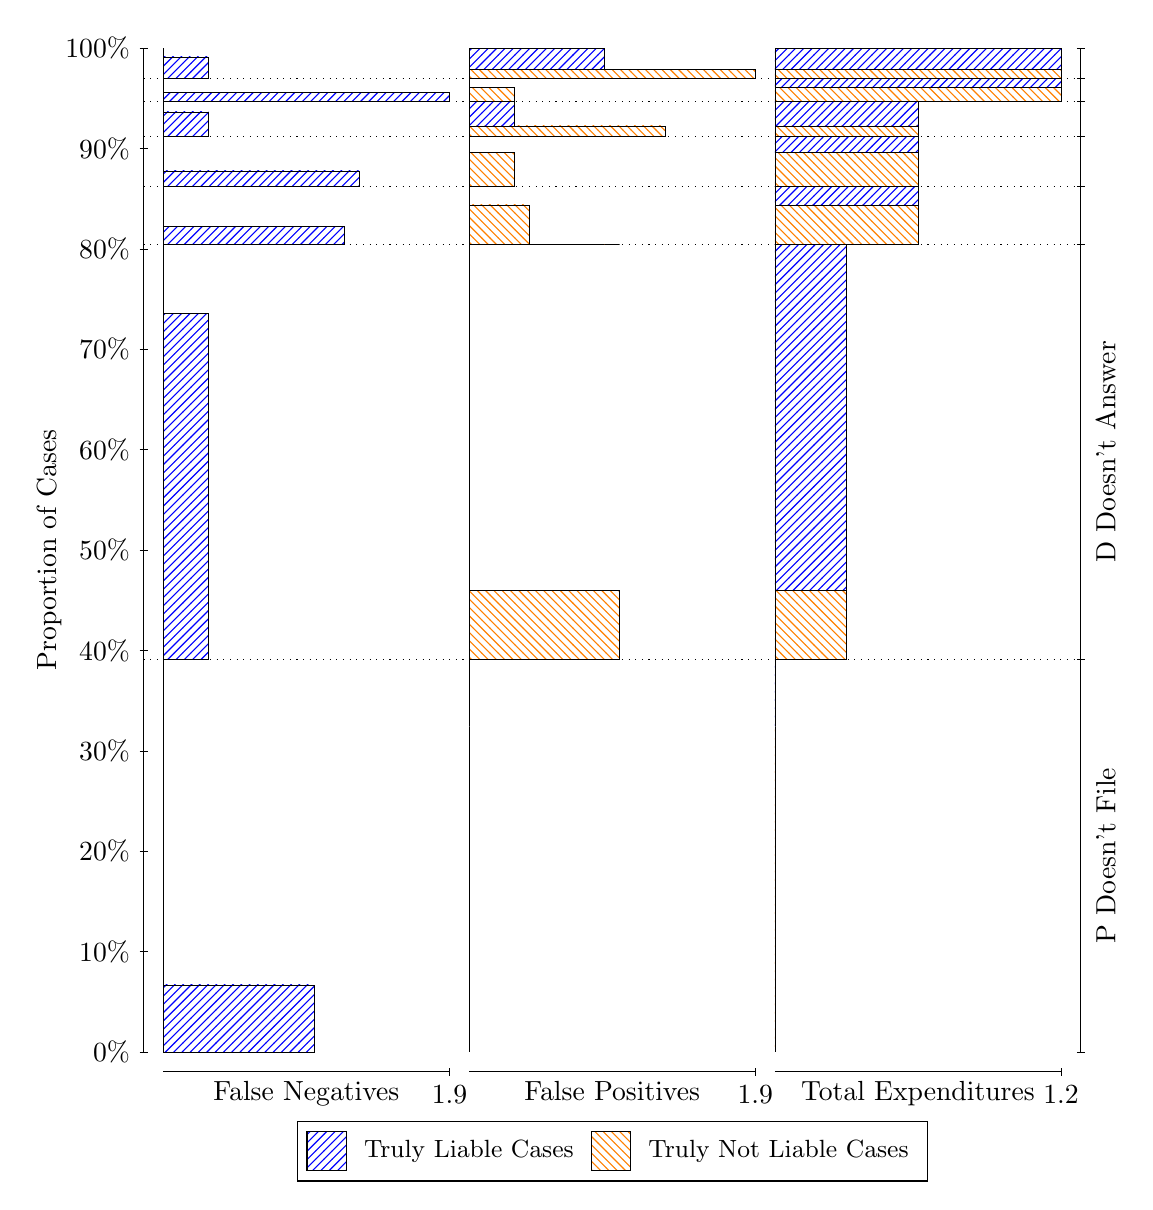
\begin{tikzpicture}
\draw[black, very thin] (1.5,1.75) -- (1.5,14.5);
\node[rotate=90, anchor=center] at (0.3, 8.125) {Proportion of Cases};
\draw[black, very thin] (1.45,1.75) -- (1.55,1.75);
\node[anchor=east] at (1.45, 1.75) {0\%};
\draw[black, very thin] (1.45,3.025) -- (1.55,3.025);
\node[anchor=east] at (1.45, 3.025) {10\%};
\draw[black, very thin] (1.45,4.3) -- (1.55,4.3);
\node[anchor=east] at (1.45, 4.3) {20\%};
\draw[black, very thin] (1.45,5.575) -- (1.55,5.575);
\node[anchor=east] at (1.45, 5.575) {30\%};
\draw[black, very thin] (1.45,6.85) -- (1.55,6.85);
\node[anchor=east] at (1.45, 6.85) {40\%};
\draw[black, very thin] (1.45,8.125) -- (1.55,8.125);
\node[anchor=east] at (1.45, 8.125) {50\%};
\draw[black, very thin] (1.45,9.4) -- (1.55,9.4);
\node[anchor=east] at (1.45, 9.4) {60\%};
\draw[black, very thin] (1.45,10.675) -- (1.55,10.675);
\node[anchor=east] at (1.45, 10.675) {70\%};
\draw[black, very thin] (1.45,11.95) -- (1.55,11.95);
\node[anchor=east] at (1.45, 11.95) {80\%};
\draw[black, very thin] (1.45,13.225) -- (1.55,13.225);
\node[anchor=east] at (1.45, 13.225) {90\%};
\draw[black, very thin] (1.45,14.5) -- (1.55,14.5);
\node[anchor=east] at (1.45, 14.5) {100\%};

\draw[black, very thin] (13.4,1.75) -- (13.4,14.5);
\draw[black, very thin] (13.35,1.75) -- (13.45,1.75);
\node[anchor=west] at (13.35, 1.75) {};
\draw[black, very thin] (13.35,6.7352) -- (13.45,6.7352);
\node[anchor=west] at (13.35, 6.7352) {};
\draw[black, very thin] (13.35,12.006) -- (13.45,12.006);
\node[anchor=west] at (13.35, 12.006) {};
\draw[black, very thin] (13.35,12.742) -- (13.45,12.742);
\node[anchor=west] at (13.35, 12.742) {};
\draw[black, very thin] (13.35,13.377) -- (13.45,13.377);
\node[anchor=west] at (13.35, 13.377) {};
\draw[black, very thin] (13.35,13.823) -- (13.45,13.823);
\node[anchor=west] at (13.35, 13.823) {};
\draw[black, very thin] (13.35,14.114) -- (13.45,14.114);
\node[anchor=west] at (13.35, 14.114) {};
\draw[black, very thin] (13.35,14.5) -- (13.45,14.5);
\node[anchor=west] at (13.35, 14.5) {};

\draw[black, very thin, pattern color=blue, pattern=north east lines] (1.75,1.75) rectangle (3.6623,2.6025);
\draw[black, very thin, pattern color=orange, pattern=north west lines] (1.75,2.6025) rectangle (1.75,6.7352);
\draw[black, very thin, pattern color=blue, pattern=north east lines] (1.75,6.7352) rectangle (2.3237,11.126);
\draw[black, very thin, pattern color=orange, pattern=north west lines] (1.75,11.126) rectangle (1.75,12.006);
\draw[black, very thin, pattern color=blue, pattern=north east lines] (1.75,12.006) rectangle (4.0447,12.239);
\draw[black, very thin, pattern color=blue, pattern=north east lines] (1.75,12.239) rectangle (3.8535,12.239);
\draw[black, very thin, pattern color=blue, pattern=north east lines] (1.75,12.239) rectangle (3.6623,12.239);
\draw[black, very thin, pattern color=blue, pattern=north east lines] (1.75,12.239) rectangle (3.4711,12.239);
\draw[black, very thin, pattern color=blue, pattern=north east lines] (1.75,12.239) rectangle (3.4711,12.239);
\draw[black, very thin, pattern color=blue, pattern=north east lines] (1.75,12.239) rectangle (3.2798,12.239);
\draw[black, very thin, pattern color=blue, pattern=north east lines] (1.75,12.239) rectangle (3.0886,12.239);
\draw[black, very thin, pattern color=blue, pattern=north east lines] (1.75,12.239) rectangle (2.8974,12.239);
\draw[black, very thin, pattern color=orange, pattern=north west lines] (1.75,12.239) rectangle (1.75,12.742);
\draw[black, very thin, pattern color=blue, pattern=north east lines] (1.75,12.742) rectangle (4.236,12.941);
\draw[black, very thin, pattern color=orange, pattern=north west lines] (1.75,12.941) rectangle (1.75,13.377);
\draw[black, very thin, pattern color=blue, pattern=north east lines] (1.75,13.377) rectangle (2.3237,13.69);
\draw[black, very thin, pattern color=orange, pattern=north west lines] (1.75,13.69) rectangle (1.75,13.823);
\draw[black, very thin, pattern color=blue, pattern=north east lines] (1.75,13.823) rectangle (5.3833,13.936);
\draw[black, very thin, pattern color=orange, pattern=north west lines] (1.75,13.936) rectangle (1.75,14.114);
\draw[black, very thin, pattern color=blue, pattern=north east lines] (1.75,14.114) rectangle (2.3237,14.387);
\draw[black, very thin, pattern color=orange, pattern=north west lines] (1.75,14.387) rectangle (1.75,14.5);
\draw[black, very thin, pattern color=orange, pattern=north west lines] (5.6333,1.75) rectangle (5.6333,5.8827);
\draw[black, very thin, pattern color=blue, pattern=north east lines] (5.6333,5.8827) rectangle (5.6333,6.7352);
\draw[black, very thin, pattern color=orange, pattern=north west lines] (5.6333,6.7352) rectangle (7.5456,7.6158);
\draw[black, very thin, pattern color=blue, pattern=north east lines] (5.6333,7.6158) rectangle (5.6333,12.006);
\draw[black, very thin, pattern color=orange, pattern=north west lines] (5.6333,12.006) rectangle (7.5456,12.006);
\draw[black, very thin, pattern color=orange, pattern=north west lines] (5.6333,12.006) rectangle (7.3544,12.006);
\draw[black, very thin, pattern color=orange, pattern=north west lines] (5.6333,12.006) rectangle (7.1632,12.006);
\draw[black, very thin, pattern color=orange, pattern=north west lines] (5.6333,12.006) rectangle (6.9719,12.006);
\draw[black, very thin, pattern color=orange, pattern=north west lines] (5.6333,12.006) rectangle (6.7807,12.006);
\draw[black, very thin, pattern color=orange, pattern=north west lines] (5.6333,12.006) rectangle (6.5895,12.006);
\draw[black, very thin, pattern color=orange, pattern=north west lines] (5.6333,12.006) rectangle (6.3982,12.509);
\draw[black, very thin, pattern color=blue, pattern=north east lines] (5.6333,12.509) rectangle (5.6333,12.742);
\draw[black, very thin, pattern color=orange, pattern=north west lines] (5.6333,12.742) rectangle (6.207,13.178);
\draw[black, very thin, pattern color=blue, pattern=north east lines] (5.6333,13.178) rectangle (5.6333,13.377);
\draw[black, very thin, pattern color=orange, pattern=north west lines] (5.6333,13.377) rectangle (8.1193,13.51);
\draw[black, very thin, pattern color=blue, pattern=north east lines] (5.6333,13.51) rectangle (6.207,13.823);
\draw[black, very thin, pattern color=orange, pattern=north west lines] (5.6333,13.823) rectangle (6.207,14.001);
\draw[black, very thin, pattern color=blue, pattern=north east lines] (5.6333,14.001) rectangle (5.6333,14.114);
\draw[black, very thin, pattern color=orange, pattern=north west lines] (5.6333,14.114) rectangle (9.2667,14.227);
\draw[black, very thin, pattern color=blue, pattern=north east lines] (5.6333,14.227) rectangle (7.3544,14.5);
\draw[black, very thin, pattern color=orange, pattern=north west lines] (9.5167,1.75) rectangle (9.5167,5.8827);
\draw[black, very thin, pattern color=blue, pattern=north east lines] (9.5167,5.8827) rectangle (9.5167,6.7352);
\draw[black, very thin, pattern color=orange, pattern=north west lines] (9.5167,6.7352) rectangle (10.425,7.6158);
\draw[black, very thin, pattern color=blue, pattern=north east lines] (9.5167,7.6158) rectangle (10.425,12.006);
\draw[black, very thin, pattern color=orange, pattern=north west lines] (9.5167,12.006) rectangle (11.333,12.006);
\draw[black, very thin, pattern color=blue, pattern=north east lines] (9.5167,12.006) rectangle (11.333,12.006);
\draw[black, very thin, pattern color=orange, pattern=north west lines] (9.5167,12.006) rectangle (11.333,12.509);
\draw[black, very thin, pattern color=blue, pattern=north east lines] (9.5167,12.509) rectangle (11.333,12.742);
\draw[black, very thin, pattern color=orange, pattern=north west lines] (9.5167,12.742) rectangle (11.333,12.742);
\draw[black, very thin, pattern color=blue, pattern=north east lines] (9.5167,12.742) rectangle (11.333,12.742);
\draw[black, very thin, pattern color=orange, pattern=north west lines] (9.5167,12.742) rectangle (11.333,13.178);
\draw[black, very thin, pattern color=blue, pattern=north east lines] (9.5167,13.178) rectangle (11.333,13.377);
\draw[black, very thin, pattern color=orange, pattern=north west lines] (9.5167,13.377) rectangle (11.333,13.51);
\draw[black, very thin, pattern color=blue, pattern=north east lines] (9.5167,13.51) rectangle (11.333,13.823);
\draw[black, very thin, pattern color=orange, pattern=north west lines] (9.5167,13.823) rectangle (13.15,14.001);
\draw[black, very thin, pattern color=blue, pattern=north east lines] (9.5167,14.001) rectangle (13.15,14.114);
\draw[black, very thin, pattern color=orange, pattern=north west lines] (9.5167,14.114) rectangle (13.15,14.227);
\draw[black, very thin, pattern color=blue, pattern=north east lines] (9.5167,14.227) rectangle (13.15,14.5);
\draw[black, dotted] (1.5,6.7352) -- (13.4,6.7352);
\draw[black, dotted] (1.5,12.006) -- (13.4,12.006);
\draw[black, dotted] (1.5,12.742) -- (13.4,12.742);
\draw[black, dotted] (1.5,13.377) -- (13.4,13.377);
\draw[black, dotted] (1.5,13.823) -- (13.4,13.823);
\draw[black, dotted] (1.5,14.114) -- (13.4,14.114);
\draw[black, very thin] (1.75,1.5) -- (5.3833,1.5);
\node[anchor=north] at (3.5667, 1.5) {False Negatives};
\draw[black, very thin] (5.3833,1.45) -- (5.3833,1.55);
\node[anchor=north] at (5.3833, 1.45) {1.9};

\draw[black, very thin] (5.6333,1.5) -- (9.2667,1.5);
\node[anchor=north] at (7.45, 1.5) {False Positives};
\draw[black, very thin] (9.2667,1.45) -- (9.2667,1.55);
\node[anchor=north] at (9.2667, 1.45) {1.9};

\draw[black, very thin] (9.5167,1.5) -- (13.15,1.5);
\node[anchor=north] at (11.333, 1.5) {Total Expenditures};
\draw[black, very thin] (13.15,1.45) -- (13.15,1.55);
\node[anchor=north] at (13.15, 1.45) {1.2};

\node[black, centered, rotate=90] at (13.72, 4.2426) {P Doesn't File};
\node[black, centered, rotate=90] at (13.72, 9.3707) {D Doesn't Answer};






\draw (7.449999999999999,1.5) node[draw=none] (baseCoordinate) {};
\begin{scope}[align=center]
        \matrix[scale=0.5, draw=black, below=0.5cm of baseCoordinate, nodes={draw}, column sep=0.1cm]{
            \node[rectangle, draw, minimum width=0.5cm, minimum height=0.5cm, pattern=north east lines, pattern color=blue] {}; &
            \node[draw=none, font=\small] (B) {Truly Liable Cases}; &
            \node[rectangle, draw, minimum width=0.5cm, minimum height=0.5cm, pattern=north west lines, pattern color=orange] {}; &
            \node[draw=none, font=\small] (B) {Truly Not Liable Cases}; \\
            };
\end{scope}

\end{tikzpicture}
\end{document}